\documentclass{standalone}


\usepackage{tikz}
\usetikzlibrary{shapes.geometric, arrows}
\usetikzlibrary{positioning}


\tikzstyle{startstop} = [rectangle, rounded corners, minimum width=2cm, minimum
height=0.5cm,text centered, draw=black]

\tikzstyle{io} = [trapezium, trapezium left angle=70, trapezium right angle=110, minimum
width=2.5cm, minimum height=0.5cm, text centered, text width = 1.5cm, draw=black]

\tikzstyle{process} = [rectangle, minimum width=2cm, minimum height=0.5cm, text centered,
text width = 1cm, draw=black]
\tikzstyle{decision} = [diamond, minimum width=2cm, minimum height=0.5cm, text centered,
draw=black]

\tikzstyle{block1} = [rectangle, rounded corners, minimum width=0.5cm, minimum
height=0.25cm,text centered, draw=black]

\tikzstyle{block2} = [rectangle, rounded corners, minimum width=2.5cm, minimum
height=3.6cm,text centered, draw=black]



\tikzstyle{arrow} = [thick,->,>=stealth]



\begin{document}
\begin{tikzpicture} [node distance=1cm, thick]
  \node (APP1) [oval] {APP1};
  \node (APP2) [oval, right=of APP1] {APP2};
  \node (APP3) [oval, right=of APP2] {APP3};
  \node (API) [process, below=of APP2, minimum width=7.5cm] {API}; 
  \node (kernel) [startstop, below=of API, minimum width=7.5cm,   label={[anchor=south
    east, inner sep=1.5pt]south east:$Kernel$}] {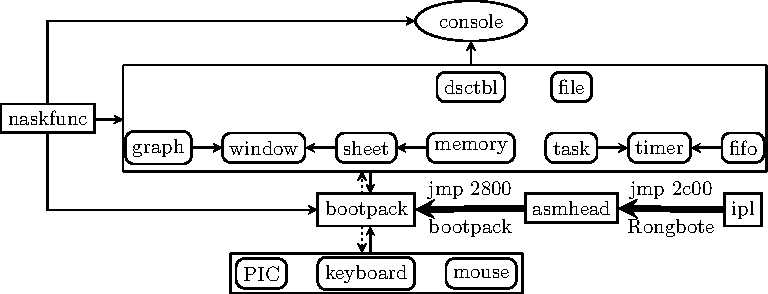
\includegraphics[width=.8\textwidth]{kernel.pdf}};
  \node (hardware) [process, below=of kernel, minimum width=7.5cm] {Hardware};
  \node (B) [below right=of hardware, xshift=-1cm, yshift=0.8cm]{B};
  \node (A) [left=of B] {A};
  \node (C) [below=of A, yshift=1cm] {A};
  \node (D) [below=of B, yshift=1cm] {B};
  \node (E) [below=of C, yshift=0.9cm] {A};
  \node (F) [below=of D, yshift=0.9cm] {B};
  

  \draw[arrow, line width= 0.9mm](E) -- node[below]{Running}(F);
  \draw[arrow] ($(APP1.south) + (-1em, 0.2em)$) -- ($(API.north) +
  (-8.55em, 0)$);
  \draw[dotArrow] ($(API.north) + (-6.55em, 0)$) -- ($(APP1.south) + (1em, .2em)$);
  \draw[arrow] ($(APP2.south) + (-1em, 0.2em)$) -- ($(API.north) + (-1em,
  0em)$);
  \draw[dotArrow] ($(API.north) + (1em, 0em)$) -- ($(APP2.south) + (1em, 0.2em)$);
  \draw[arrow] ($(APP3.south) + (-1em, 0.2em)$) -- ($(API.north) + (6.55em, 0em)$);
  \draw[dotArrow]($(API.north) + (8.55em, 0em)$) -- ($(APP3.south) + (1em, 0.2em)$);
  \draw[arrow] ($(API.south) + (-1em, 0)$) -- ($(kernel.north) + (-1em, 0)$);
  \draw[dotArrow] ($(kernel.north) + (1em, 0em)$) -- ($(API.south) + (1em, 0em)$);
  \draw[arrow] ($(kernel.south) + (-1em, 0em)$) -- ($(hardware.north) + (-1em, 0em)$);
  \draw[dotArrow] ($(hardware.north) + (1em, 0em)$) -- ($(kernel.south) + (1em, 0)$);
  \draw[arrow] (A) -- node[below]{Call}(B);
  \draw[dotArrow] (C) -- node[below]{Service}(D);
\end{tikzpicture}


\end{document}



%%% Local Variables:
%%% mode: latex
%%% TeX-master: t
%%% End:
